\chapter{Method}\label{cha:method}
This chapter will give a detailed description on which how the problem real-time text rendering on mobile devices was solved in this thesis. This chapter is divided into two different parts. The first part gives a detailed description about the implementation of the distance transform module. This part has been reimplemented several times due to poor performance. The second part gives a detailed description about the implementation of the distance field rendering module.

\section{Distance field generation initial attempt}
There is many EDT algorithms for creating distance fields. Most of the EDT algorithms used today runs in $\mathcal{O}(nm)$, where n and m are the width respectively the height of the image. Example of algorithms running in $\mathcal{O}(nm)$ are \citet{Danielsson} and \citet{meijster}.

The initial implementation of distance field generation in this thesis was built around \citet{Gustavson:2011} article on the subject. A signed version of the 8SED algorithm was used along with the anti-aliased sub-pixel distance measure proposed in the article. A signed distance field has several advantages compared to an unsigned distance field. The most obvious advantages is the increased flexibility it gives and that it facilitates the implementation of proper anti-aliasing on the border of the shape due to the increased information in an environment around the border pixels\citep{gustavson20122d}. To generate a signed distance field the distance transform was run twice with inverted input representation. This will make one of the transforms create a distance field on the inside of the glyph and the other transform on the outside of the glyph. The resulting distance field was then calculated with the following formula.\vspace{\baselineskip}\newline
$result(i,j) = inside(i,j) - outside(i,j), \forall (i, j), i \in \{0,\dots, m-1\}, j \in \{0,\dots, n-1\}$ \vspace{\baselineskip}\newline
\section{Fast and approximate distance field generation}
Fast distance field generation on mobile devices requires some approximations and optimizations to decrease the transformation time. This can be seen in many of the of the distance field generation implementations done lately. Two examples of this is GLyphy by Behdad Esfahbod and the implementation of distance field generation in QT. Both the implementations approximate the bezier curves from the font file to some different representation of a glyph that is easier to work with. GLyphy approximates the bezier curves to circular arcs and QT approximates the bezier curves to line segments. This makes it possible to draw distance fields locally over the outlines of the glyph and a distance transform of the whole image is not needed.

Because the initial implementation of the distance field generation was too slow to meet the requirement another faster implementation was necessary. A variant of the implementation done by Qt was implemented. The implementation was divided into four steps in the following order, extracting beziers from the given font file, approximating the beziers to line segments, drawing the glyph in an image and drawing distance gradients over the line segments to create a distance field locally over the outlines of the glyph. Extraction of bezier curves from font files can easily be done with different libraries for example freetype and a description of how this is done is not relevant for the proceeding of this report. 
\subsection{Bezier to line segment approximations}
Bezier to line segment approximations is done alot in computer graphics and can be done by using the properties of the de Casteljau's algorithm. A naive way to solve the beziér to line segment problem is to split the Beziér curve into $n$ smaller curves with a constant length and approximate them to line segments. This would make the line density constant over the whole curve meaning that both the strongly bent parts and the almost straight parts will be represented by equally many line segments. A smarter way to solve this is proposed in an article by \citet{fischer2000} which involves using a recursive function dividing the bezier into two parts until a stop condition is met. This will make the line segment density higher where the curve is strongly bent and lower where the curve is almost straight. The following pseudocode is taken from the article by Fischer.
\begin{algorithm}[H]
\caption{Function for approximating beziér to line segment}
\begin{algorithmic}
\Procedure{flattenCurve}{Curve c}
\If {\Call{isSufficientlyFlat}{c}}
  \State output(c);
\Else
	\State Curve l,r\;
	\State\Call{subdivide}{c,l,r}\;
	\State\Call{flattenCurve}{l}\;
	\State\Call{flattenCurve}{r}\;
\EndIf
\EndProcedure
\end{algorithmic}
\end{algorithm}
In the above code the type Curve is a beziér curve for example a cubic bezier curve represented by 4 points in the plane or a cubic beziér represented by 3 points in the plane. The 2 functions isSufficientlyFlat and subdivide is not defined in the above code because the implementation of them differs depending on the curve type used. The function isSufficientlyFlat checks the difference between the curve and the line segment from the start point to the endpoint of the curve is small enough to meet the stop condition. This function can be implemented in many different ways. In his article Fischer propose solution for cubic beziérs initially developed by Roger Willcocks. The pseudocode for this solution follows.

\begin{algorithm}[H]
\caption{Stop condition for cubic beziér subdivision}
\begin{algorithmic}
\Function{isSufficientlyFlat}{Curve c}
	\State double ux = 3.0*c.b1.x - 2.0*c.b0.x - c.b3.x; ux *= ux\;
	\State double uy = 3.0*c.b1.y - 2.0*c.b0.y - c.b3.y; uy *= uy\;
	\State double vx = 3.0*c.b2.x - 2.0*c.b3.x - c.b0.x; vx *= vx\;
	\State double vy = 3.0*c.b2.y - 2.0*c.b3.y - c.b0.y; vy *= vy\;
	\If{ux<vx} 
	\State ux = vx\; 	
	\EndIf
	\If{uy<vy} 
		\State uy = vy\; 
	\EndIf
	\State\Return (ux+uy $\leq$ tolerance)\;
\EndFunction
\end{algorithmic}
\end{algorithm}

There are other ways to check if a curve is flat enough to approximate it to a line segment. One solution is proposed by \citet{bezier_subdivision}. The stop condition in his article only depends on the distance between the two points $P_1$ and $P_2$ and the line between $P_0$ and $P_4$.

The function subdivide in the algorithm for approximating beziers to line segments proposed by Fischer is implemented using the special case of de Casteljau's algorithm splitting at $t=0.5$.  
%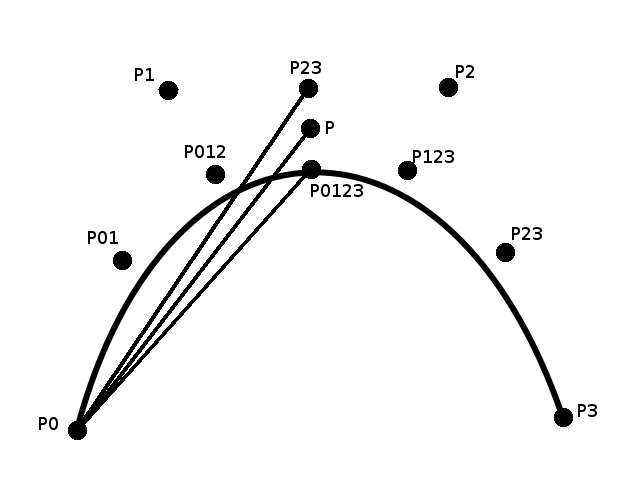
\includegraphics[scale=0.5]{bezier_pused}
\subsection{Drawing the glyph}
The distance gradients in the distance field will only be drawn locally withing a predefined distance from each outline. This creates a need to draw the glyph in the image before generating the distance field. If the glyph is not drawn before the distance gradients are drawn there will most certainly be parts of the glyph that have the outside color but is located on the inside of the glyph. For example the middle of the 'I' might be the same color as pixels outside the glyph. This would lead to a hole in the middle of the 'I' when rendering it which is not desired. The input to this step of the distance field generation is a glyph represented as connected line segments in the shape of a polygon. As mentioned in the background the scan-line algorithm together with the odd even fill rule or the non-zero winding rule can be used to fill a polygon. Because is a very common problem in computer graphics and there are many open source libraries doing this very fast and optimized there was no need to implement this. To solve this the function drawPath in the open source 2D graphics library Skia was used. The Skia library was already installed and used in other places within Visiarc's products.
\subsection{Drawing distance gradients}
Drawing gradients can be done in many different ways. The initial implementation of this step had real measured distances as values in each pixel in the gradient. Description of how the pixel to line segment distance was measured follows. The pixel coordinate was projected onto the line. If the projection hit the line the distance was equal to the projection distance. Otherwise the distance was equal to the shortest distance to one of the endpoints of the line.

\begin{figure}[H]
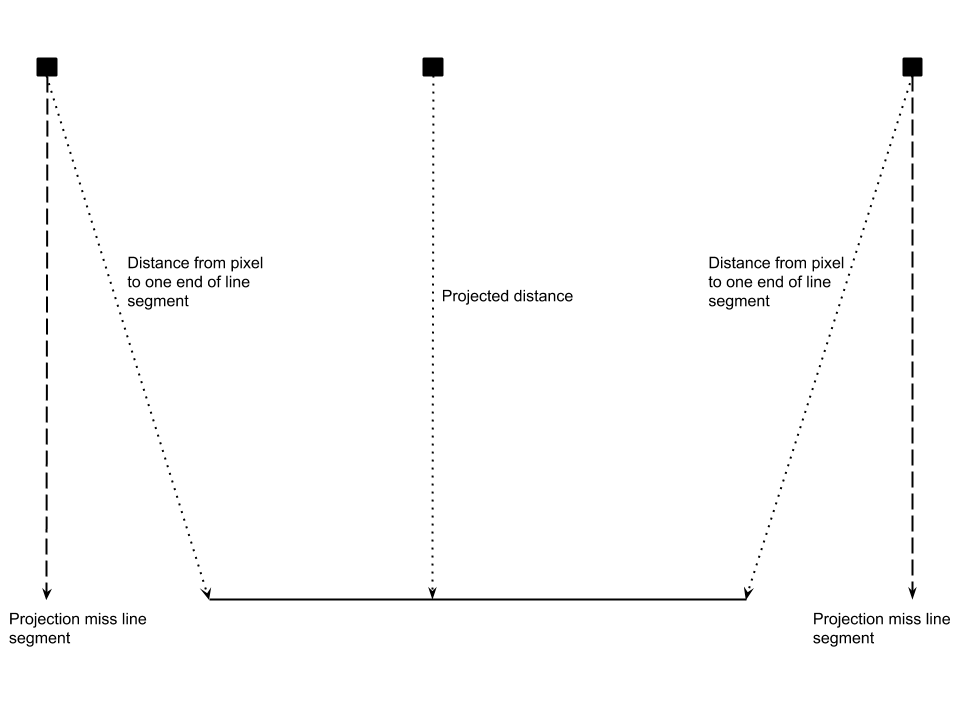
\includegraphics[scale=0.35]{pixel_line_measure}
\caption{Shortest distance from pixel to line segment}
\end{figure}

The code for projecting a pixel to a line segment made the distance fields look good because there was few sources of errors drawing the gradients. Every pixel was calculated independently from eachother and if the new distance was not better than the distance already in the pixel the pixel was not updated. The only problem with this approach was the execution time. The code for pixel to line segmen distance calculation was located in the innermost loop which means that the code was executed very many times and performance improvements was neccessary.

In the distance field generation made by Qt no pixel to line projection is done. They draw the gradient directly using trigonometry stepping through the pixels row by row. This influenced how the gradients is drawn in the final result of this thesis. Every line segment will result in two gradients drawn, one rectangular over the line and one triangular close to the first end points of the line segment. The gradients drawn for line segment A and B is illustrated in figureXXX.

\begin{figure}[H]
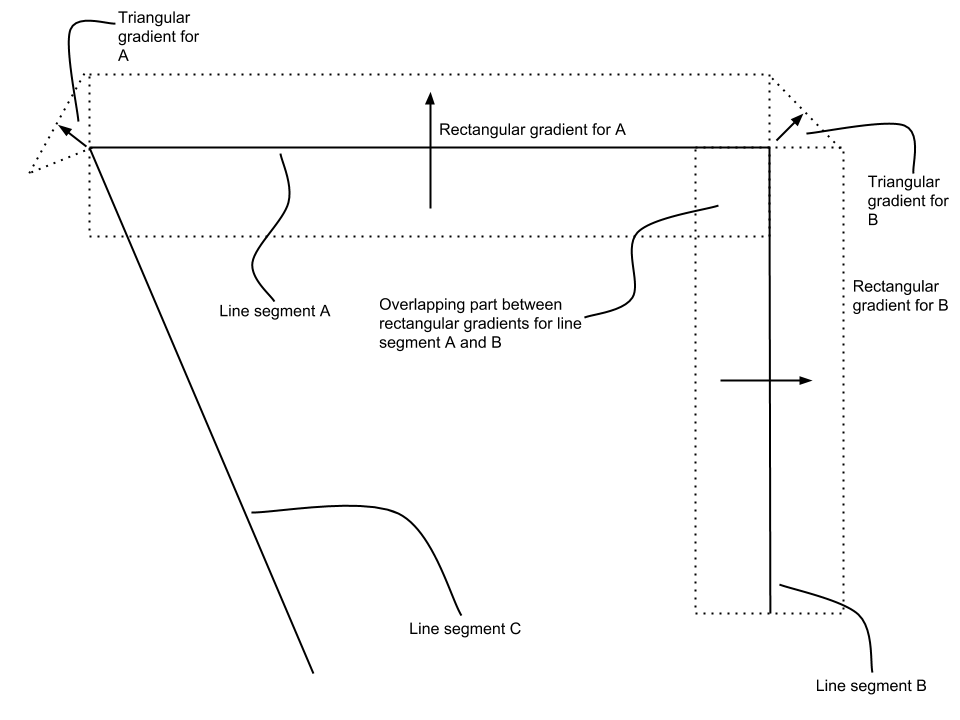
\includegraphics[scale=0.35]{gradient_drawing}
\caption{Illustration of the drawn gradients for line segment A and B}
\end{figure}

There are some troublesome areas in the distance field around the line segment connections. One of the troublesome areas is the overlapping area between line segment A and line segment B. A naive approach using this solution would paint the gradient for line segment A first and then paint the gradient for line segment B. This would result in parts of the gradient for line segment A being overwritten. To solve this a check is done before every write. For inside pixels a write is only permitted if the new value is higher than the current value and for outside pixels a write is only permitted if the new value is lower than the current value. Another problem that will occur if two line segments is not perpendicular

\begin{figure}[H]
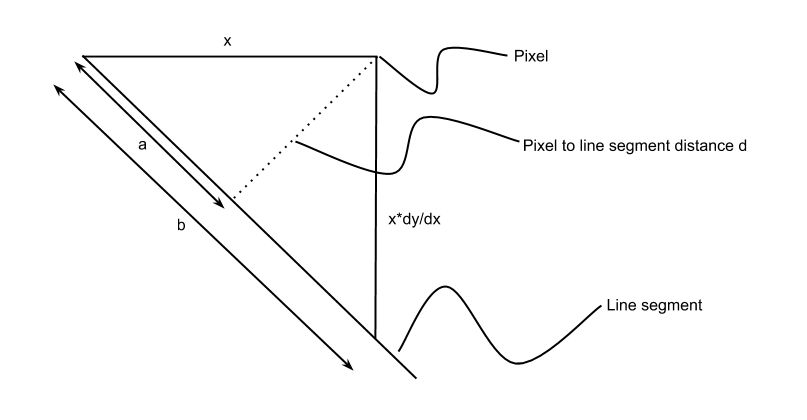
\includegraphics[scale=0.5]{draw_gradient}
\caption{Illustration of the calculations done when drawing the gradient}
\end{figure}

The line segment is defined between two points in the plane $p_1$ and $p_2$. The derivative of the line can trivially be calculated $\frac{dy}{dx}=\frac{p_{2y}-p_{1y}}{p_{2x}-p_{1x}}$. The projection of the pixel to the line segment will always be perpendicular to the line segment. This implies that the triangle with sides $x$, $x\frac{dy}{dx}$ and $b$ and the triangle with sides $x$, $a$ and $d$ are similar triangles which means that $\frac{x}{b}=\frac{a}{x\frac{dy}{dx}}=\frac{d}{x}$ is true. The similarity of the triangles means that $d$ can be calculated in two ways, either $d=\frac{x^2}{b}$ or $d=\frac{a}{\frac{dy}{dx}}$. The first solution is used in the thesis because b is easier to calculate than a $b=\sqrt{x^2+(x*\frac{dy}{dx})^2}$. Having $b$ the final formula for calculating d is $d=\frac{x^2}{\sqrt{x^2+(x*\frac{dy}{dx})^2}}=\frac{x}{\sqrt{1+\frac{dy}{dx}^2}}$. The shortest distance from the line segment to the pixel is equal to $|d|$.
